
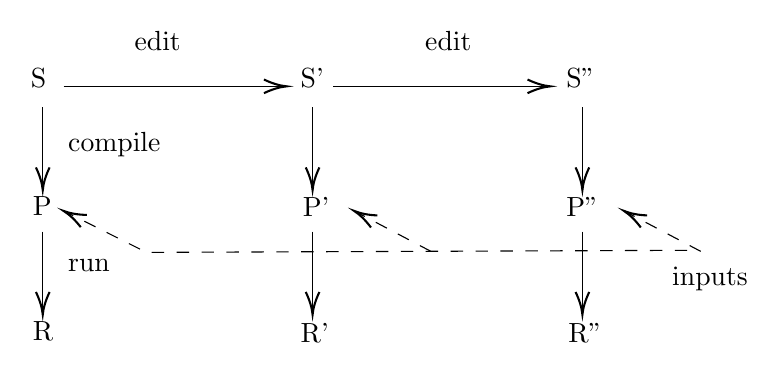
\begin{tikzpicture}[x=0.75pt,y=0.75pt,yscale=-1,xscale=1]
%uncomment if require: \path (0,300); %set diagram left start at 0, and has height of 300

%Straight Lines [id:da15853117718106668] 
\draw    (70,50) -- (175.5,50) ;
\draw [shift={(177.5,50)}, rotate = 180] [color={rgb, 255:red, 0; green, 0; blue, 0 }  ][line width=0.75]    (10.93,-3.29) .. controls (6.95,-1.4) and (3.31,-0.3) .. (0,0) .. controls (3.31,0.3) and (6.95,1.4) .. (10.93,3.29)   ;
%Straight Lines [id:da652672843484112] 
\draw    (60,60) -- (60,98) ;
\draw [shift={(60,100)}, rotate = 270] [color={rgb, 255:red, 0; green, 0; blue, 0 }  ][line width=0.75]    (10.93,-3.29) .. controls (6.95,-1.4) and (3.31,-0.3) .. (0,0) .. controls (3.31,0.3) and (6.95,1.4) .. (10.93,3.29)   ;
%Straight Lines [id:da11336367015023918] 
\draw    (190,60) -- (190,98) ;
\draw [shift={(190,100)}, rotate = 270] [color={rgb, 255:red, 0; green, 0; blue, 0 }  ][line width=0.75]    (10.93,-3.29) .. controls (6.95,-1.4) and (3.31,-0.3) .. (0,0) .. controls (3.31,0.3) and (6.95,1.4) .. (10.93,3.29)   ;
%Straight Lines [id:da9768188564067921] 
\draw    (200,50) -- (302.5,50) ;
\draw [shift={(304.5,50)}, rotate = 180] [color={rgb, 255:red, 0; green, 0; blue, 0 }  ][line width=0.75]    (10.93,-3.29) .. controls (6.95,-1.4) and (3.31,-0.3) .. (0,0) .. controls (3.31,0.3) and (6.95,1.4) .. (10.93,3.29)   ;
%Straight Lines [id:da5343007964966324] 
\draw    (320,60) -- (320,98) ;
\draw [shift={(320,100)}, rotate = 270] [color={rgb, 255:red, 0; green, 0; blue, 0 }  ][line width=0.75]    (10.93,-3.29) .. controls (6.95,-1.4) and (3.31,-0.3) .. (0,0) .. controls (3.31,0.3) and (6.95,1.4) .. (10.93,3.29)   ;
%Straight Lines [id:da5682106363637645] 
\draw    (60,120) -- (60,158) ;
\draw [shift={(60,160)}, rotate = 270] [color={rgb, 255:red, 0; green, 0; blue, 0 }  ][line width=0.75]    (10.93,-3.29) .. controls (6.95,-1.4) and (3.31,-0.3) .. (0,0) .. controls (3.31,0.3) and (6.95,1.4) .. (10.93,3.29)   ;
%Straight Lines [id:da21653990085554842] 
\draw    (190,120) -- (190,158) ;
\draw [shift={(190,160)}, rotate = 270] [color={rgb, 255:red, 0; green, 0; blue, 0 }  ][line width=0.75]    (10.93,-3.29) .. controls (6.95,-1.4) and (3.31,-0.3) .. (0,0) .. controls (3.31,0.3) and (6.95,1.4) .. (10.93,3.29)   ;
%Straight Lines [id:da6880192453985609] 
\draw    (320,120) -- (320,158) ;
\draw [shift={(320,160)}, rotate = 270] [color={rgb, 255:red, 0; green, 0; blue, 0 }  ][line width=0.75]    (10.93,-3.29) .. controls (6.95,-1.4) and (3.31,-0.3) .. (0,0) .. controls (3.31,0.3) and (6.95,1.4) .. (10.93,3.29)   ;
%Straight Lines [id:da4584594487312068] 
\draw  [dash pattern={on 4.5pt off 4.5pt}]  (370.5,129) -- (110,130) -- (71.79,110.89) ;
\draw [shift={(70,110)}, rotate = 26.57] [color={rgb, 255:red, 0; green, 0; blue, 0 }  ][line width=0.75]    (10.93,-3.29) .. controls (6.95,-1.4) and (3.31,-0.3) .. (0,0) .. controls (3.31,0.3) and (6.95,1.4) .. (10.93,3.29)   ;
%Straight Lines [id:da01744371715533921] 
\draw  [dash pattern={on 4.5pt off 4.5pt}]  (247,129.5) -- (211.77,110.93) ;
\draw [shift={(210,110)}, rotate = 27.79] [color={rgb, 255:red, 0; green, 0; blue, 0 }  ][line width=0.75]    (10.93,-3.29) .. controls (6.95,-1.4) and (3.31,-0.3) .. (0,0) .. controls (3.31,0.3) and (6.95,1.4) .. (10.93,3.29)   ;
%Straight Lines [id:da36809290332362665] 
\draw  [dash pattern={on 4.5pt off 4.5pt}]  (377,129.5) -- (341.77,110.93) ;
\draw [shift={(340,110)}, rotate = 27.79] [color={rgb, 255:red, 0; green, 0; blue, 0 }  ][line width=0.75]    (10.93,-3.29) .. controls (6.95,-1.4) and (3.31,-0.3) .. (0,0) .. controls (3.31,0.3) and (6.95,1.4) .. (10.93,3.29)   ;

% Text Node
\draw (54,102) node [anchor=north west][inner sep=0.75pt]   [align=left] {P};
% Text Node
\draw (53,40) node [anchor=north west][inner sep=0.75pt]   [align=left] {S};
% Text Node
\draw (184,102) node [anchor=north west][inner sep=0.75pt]   [align=left] {P'};
% Text Node
\draw (183,40) node [anchor=north west][inner sep=0.75pt]   [align=left] {S'};
% Text Node
\draw (311,102) node [anchor=north west][inner sep=0.75pt]   [align=left] {P''};
% Text Node
\draw (311,40) node [anchor=north west][inner sep=0.75pt]   [align=left] {S''};
% Text Node
\draw (71,71) node [anchor=north west][inner sep=0.75pt]   [align=left] {compile};
% Text Node
\draw (103,22) node [anchor=north west][inner sep=0.75pt]   [align=left] {edit};
% Text Node
\draw (243,22) node [anchor=north west][inner sep=0.75pt]   [align=left] {edit};
% Text Node
\draw (71,132) node [anchor=north west][inner sep=0.75pt]   [align=left] {run};
% Text Node
\draw (54,162) node [anchor=north west][inner sep=0.75pt]   [align=left] {R};
% Text Node
\draw (183,163) node [anchor=north west][inner sep=0.75pt]   [align=left] {R'};
% Text Node
\draw (312,163) node [anchor=north west][inner sep=0.75pt]   [align=left] {R''};
% Text Node
\draw (362,136) node [anchor=north west][inner sep=0.75pt]   [align=left] {inputs};


\end{tikzpicture}
